
\begin{frame}{‌مسئلهٔ پوشش رأسی}
\begin{itemize}\itemr
\item[-]
مسئله پوشش رأسی
\fn{1}{vertex cover problem}
یک مسئلهٔ ان‌پی کامل است.
\item[-]
پوشش رأسی یک گراف بدون جهت
\m{G = (V,E)}
زیر مجموعه‌ای از رئوس گراف
\m{V' \subseteq V}
است به طوری‌که اگر
\m{(u,v)}
یک یال از گراف
\m{G}
باشد، آنگاه
\m{u \in V'}
یا
\m{v \in V'}
یا هردو. اندازه پوشش رأسی تعداد رأس‌های زیر مجموعهٔ
\m{V'}
است.
\item[-]
در مسئلهٔ پوشش رأسی می‌خواهیم کمترین تعداد رئوس در یک گراف را پیدا کنیم که یک پوشش رأسی تشکیل می‌دهند یا به عبارت دیگر همهٔ یال‌ها را پوشش می دهند. به چنین پوشش رأسی یک پوشش رأسی بهینه
\fn{2}{optimal vertex cover}
می‌گوییم.
\item[-]
اگرچه هیچ الگوریتم چند جمله‌ای برای مسئلهٔ پوشش رأسی یافته نشده است، اما یک الگوریتم تقریبی چندجمله‌ای برای پیدا کردن جواب نزدیک به بهینه وجود دارد.
\end{itemize}
\end{frame}


\begin{frame}{‌مسئلهٔ پوشش رأسی}
\begin{itemize}\itemr
\item[-]
الگوریتم تقریبی زیر یک گراف بدون جهت را دریافت می‌کند و یک پوشش رأسی باز می‌گرداند که اندازهٔ آن کمتر از دو برابر پوشش رأسی بهینه است.
\begin{algorithm}[H]\alglr
  \caption{Approx-Vertex-Cover} 
  \begin{algorithmic}[1]
   \Func{Approx-Vertex-Cover}{G}
   \State C = $\emptyset$
   \State E' = G.E
   \While{E' $\neq \emptyset$}
   			\State let (u,v) be an arbitrary edge of E'
   			\State C = C $\cup$ \{(u,v)\}
   			\State remove from E' edge (u,v) and every edge incident on either u or v
   	\EndWhile
   	\State \Return C                      
  \end{algorithmic}
  \label{alg:merge}
\end{algorithm}
\item[-]
متغیر
\m{C}
پوشش رأسی تشکیل شده را در بر می‌گیرد. این الگوریتم در زمان
\m{O(|V|+|E|)}
توسط نمایش گراف با لیست مجاورت اجرا می‌شود.
\end{itemize}
\end{frame}


\begin{frame}{‌مسئلهٔ پوشش رأسی}
\begin{itemize}\itemr
\item[-]
شکل زیر نشان می‌دهد این الگوریتم چگونه برروی یک گراف عمل می‌کند.
در پایان این الگوریتم تقریبی ۶ رأس را برای پوشش رأسی پیدا می‌کند در صورتی که جواب بهینه برای این نمونه مسئله ۳ است.
\begin{figure}
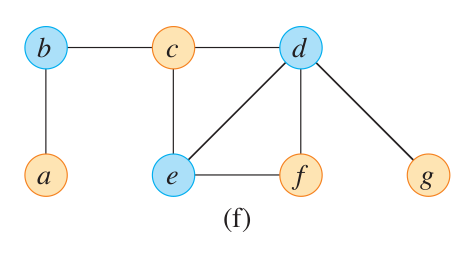
\includegraphics[width=0.3\textwidth]{figs/chap08/1108-vertex-cover-res}
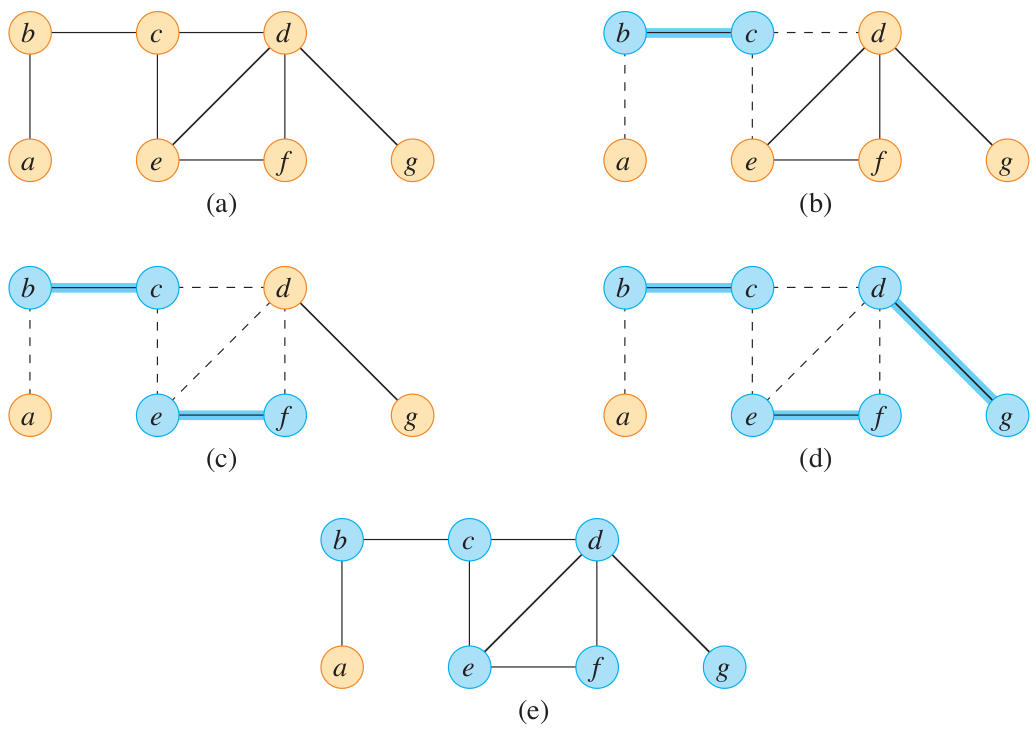
\includegraphics[width=0.6\textwidth]{figs/chap08/1108-vertex-cover}
\end{figure}
\end{itemize}
\end{frame}


\begin{frame}{‌مسئلهٔ پوشش رأسی}
\begin{itemize}\itemr
\item[-]
قضیه : الگوریتم تقریبی پوشش رأسی یک الگوریتم چند جمله‌ای تقریبی با ضریت ۲ است.
\item[-]
اثبات : مجموعهٔ
\m{C}
یک پوشش رأسی است زیرا الگوریتم در حلقه تا وقتی تکرار می‌شود که همهٔ یال‌های
\m{G.E}
با یکی از رئوس
\m{C}
پوشش داده شده‌اند.
\item[-]
حال می‌خواهیم ثابت کنیم این الگوریتم یک الگوریتم تقریبی با ضریب ۲ است.
\item[-]
فرض کنید
\m{A}
مجموعه‌ای از یال‌ها باشد که در خط ۴ الگوریتم انتخاب شده‌اند. برای اینکه یال‌های مجموعه
\m{A}
پوشش داده شوند، هر پوشش رأسی باید حداقل یکی از دو رأس هریال در
\m{A}
را شامل شود. هیچ دو یالی در
\m{A}
رأس مشترک ندارند، زیرا وقتی یک یال در خط ۴ انتخاب شد، همهٔ یال‌هایی که با آن یال رأس مشترک دارند از مجموعه
\m{E'}
در خط ۶ حذف می‌شوند.
\end{itemize}
\end{frame}


\begin{frame}{‌مسئلهٔ پوشش رأسی}
\begin{itemize}\itemr
\item[-]
بنابراین هیچ دویالی در
\m{A}
با یک رأس از
\m{C^*}
پوشش داده نشده‌اند و این بدین معنی است که به ازای هر رأس در
\m{C^*}
، حداکثر یک یال در
\m{A}
وجود دارد و بنابراین داریم :
\begin{align*}
\m{|C^*| \geqslant |A|}
\end{align*}
\item[-]
هر اجرای خط ۴ یک یال را انتخاب می‌کند که هیچ‌کدام از دو رأس مجاور آن در
\m{C}
نیستند و بنابراین داریم :
\begin{align*}
\m{|C| = 2 |A|}
\end{align*}
\item[-]
با استفاده از دو رابطهٔ به دست آمده خواهیم داشت :
\begin{align*}
\m{|C| = 2 |A| \leqslant 2|C^*|}
\end{align*}
و قضیه بدین ترتیب اثبات می‌شود.
\end{itemize}
\end{frame}